\documentclass[a4paper,11pt]{article}
\usepackage[utf8]{inputenc}
\usepackage{fullpage}
\usepackage{graphicx}
\usepackage{wrapfig}
\usepackage{caption}
\usepackage{subcaption}
\usepackage{appendix}
\usepackage{tcolorbox}
\tcbuselibrary{theorems}
\usepackage{tabularx}
\usepackage{float}
\usepackage{listings}
\usepackage{color}

\definecolor{dkgreen}{rgb}{0,0.6,0}
\definecolor{gray}{rgb}{0.5,0.5,0.5}
\definecolor{mauve}{rgb}{0.58,0,0.82}

\lstset{frame=tb,
	language=MATLAB,
	aboveskip=3mm,
	belowskip=3mm,
	showstringspaces=false,
	columns=flexible,
	basicstyle={\small\ttfamily},
	numbers=none,
	numberstyle=\tiny\color{gray},
	keywordstyle=\color{blue},
	commentstyle=\color{dkgreen},
	stringstyle=\color{mauve},
	breaklines=true,
	breakatwhitespace=true,
	tabsize=3
}

\newtcbtheorem[number within=section]{theo}{}%
{colback=green!5,colframe=green!35!black,fonttitle=\bfseries}{th}

\usepackage{hyperref}
\definecolor{navyblue}{rgb}{0.0, 0.0, 0.5}
\definecolor{myblue}{RGB}{15,77,145}
\definecolor{mountainmeadow}{rgb}{0.19, 0.73, 0.56}
\hypersetup{
	colorlinks=true,
	linkcolor=myblue,
	citecolor=mountainmeadow,
	urlcolor=navyblue,
}

\title{% 
	\textbf{4F13: Probabilistic Machine Learning} \\
	\vspace{5pt}
	\large Coursework 1: Gaussian Processes \\

	\vspace{10pt}
	\small \textit{Michaelmas 2021}}
\author{\small Oussama Chaib, oc327@cam.ac.uk}
\date{\small October 2021}

\begin{document}
	\setlength\parindent{0pt}
	\maketitle
%	\tableofcontents
%	\pagebreak
	\section*{Question (a)}
	\noindent
	The data in \texttt{cw1a.mat} is loaded and used as a training set for a Gaussian model of squared exponential covariance function and Gaussian likelihood using the initial settings described below.
	The negative marginal log likelihood of the model is then minimized and the 95\% predictive error bars are calculated from the obtained prediction data. The hyperparameters of the "optimal" fit (i.e: the model that minimises the negative marginal log likelihood) are described below, alongside the obtained function.
	\begin{table}[H]
	\centering
	\begin{tabular}{| c  | c | c | c | c |}
		\hline
		& \textbf{$l$} & $\nu$ & \textbf{$\sigma_{noise}$} & $likelihood$ \\
		\hline \hline
		\textbf{Initial} & 0.3679 & 1 & 1 & 4.4636e-41\\
		\hline
		\textbf{Predicted} & 0.1282 & 0.8970 & 0.1178 & 6.7971e-06\\
		\hline
	\end{tabular}
	\caption{Initial settings for hyperparameters}
\end{table}
\begin{figure}[H]
	\centering
	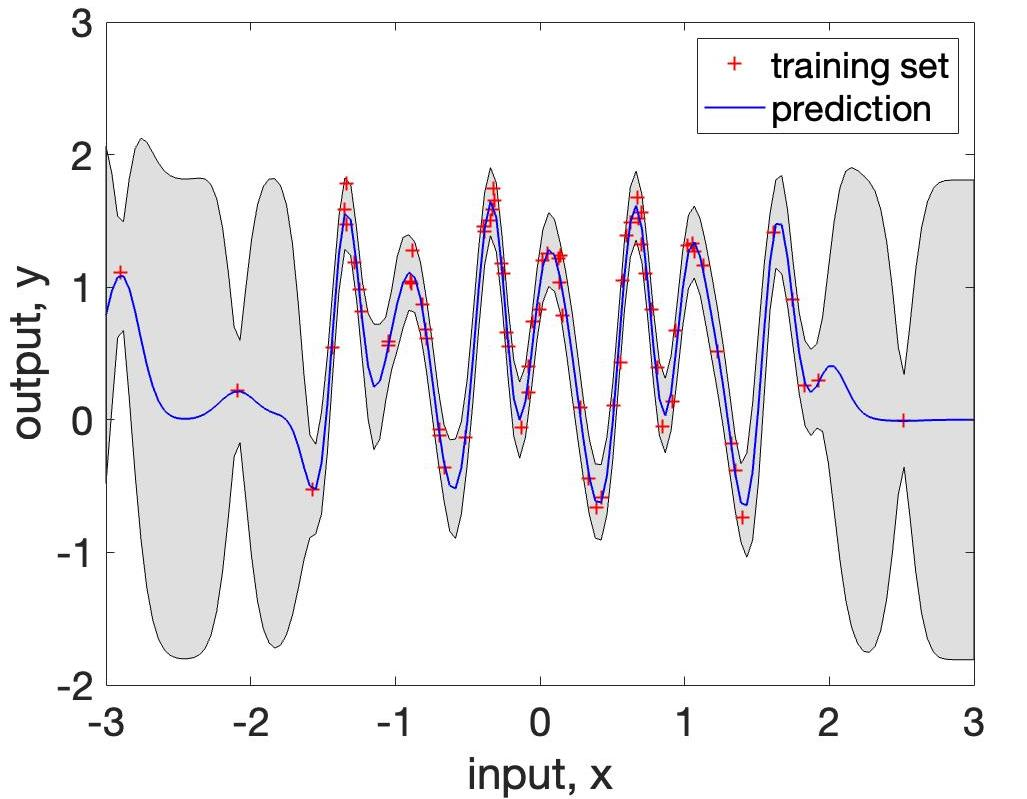
\includegraphics[width=.7\linewidth]{figures/a1.jpg}
	\caption{Training and predicted data fit using the described initial settings}
	\label{fig:1}
\end{figure}
\noindent
We observe that the predictive errorbars are higher in regions with a low number of data points, and lower in regions containing more data points. This can be explained by the characteristic lengthscale which is in this case relatively small ($l = 0.1282$), yielding a "wiggly" fit. Therefore, when points are far away from each other (i.e: by a distance higher than $l$), the correlation between them drops and that is compensated by an increase in uncertainty. We also observe that the standard deviation of the function $\nu$ is 7 to 8 times higher than the standard deviation of the noise $\sigma_{noise}$. The larger error bars are therefore most likely due to the uncertainty of the underlying function, while the contribution of noise is, in this case, smaller.
\begin{lstlisting}
	% coursework1a.m
	hyp = struct('mean', [] , 'cov', [-1,0] , 'lik', 0);
	hyp_min = minimize(hyp, @gp, -100, @infGaussLik, meanfunc, covfunc, likfunc, x, y);
	[ys stds] = gp(hyp_min, @infGaussLik, meanfunc, covfunc, likfunc, x, y, xs);
\end{lstlisting}
\section*{Question (b)}
The hyperparameters are initialised differently in this question. After trying different arbitrary values, we notice there are, \textit{a priori}, two types of "optimal" models we can get by varying the lengthscale. The first one is the same as the model shown in the previous section (\hyperref[fig:1]{\textbf{Figure 1}}). The second is represented in the graphs below.
	\begin{table}[H]
	\centering
	\begin{tabular}{| c  | c | c | c |}
		\hline
		& \textbf{$l$} & $\nu$ & \textbf{$\sigma_{noise}$} \\
		\hline \hline
		\textbf{Initial} & $e^0=1$ & 1 & 1 \\
		\hline
		\textbf{Predicted} & 8.0421 & 0.6989 & 0.6632 \\
		\hline
	\end{tabular}
	\vspace{5pt}
	\begin{tabular}{| c  | c | c | c |}
		\hline
		& \textbf{$l$} & $\nu$ & \textbf{$\sigma_{noise}$} \\
		\hline \hline
		\textbf{Initial} & $e^{10}=2.2e04$ & 1 & 1 \\
		\hline
		\textbf{Predicted} & 2.2e04 & 0.7437 & 0.6671 \\
		\hline
	\end{tabular}
	
	\caption{Hyperparameters obtained for local optima by modifying initial hyperparameters}
\end{table}
\begin{figure}[h]
	\centering
	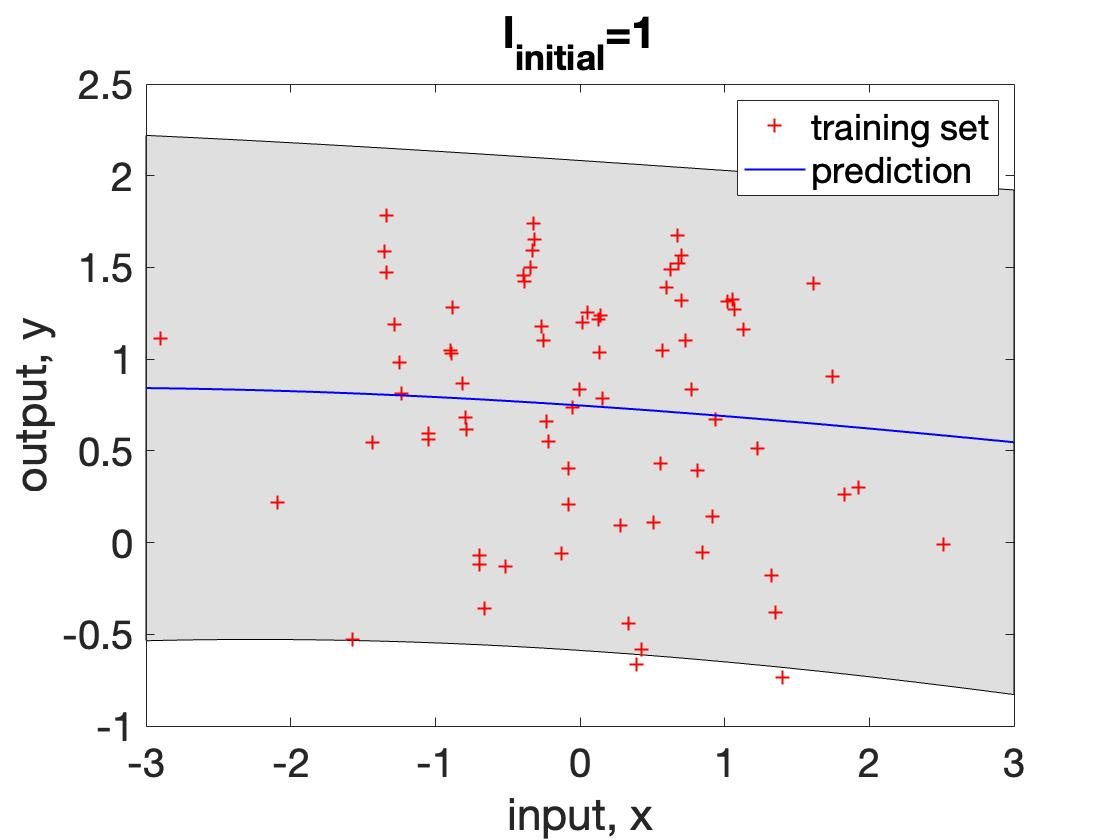
\includegraphics[width=.48\linewidth]{figures/b4.jpg}
	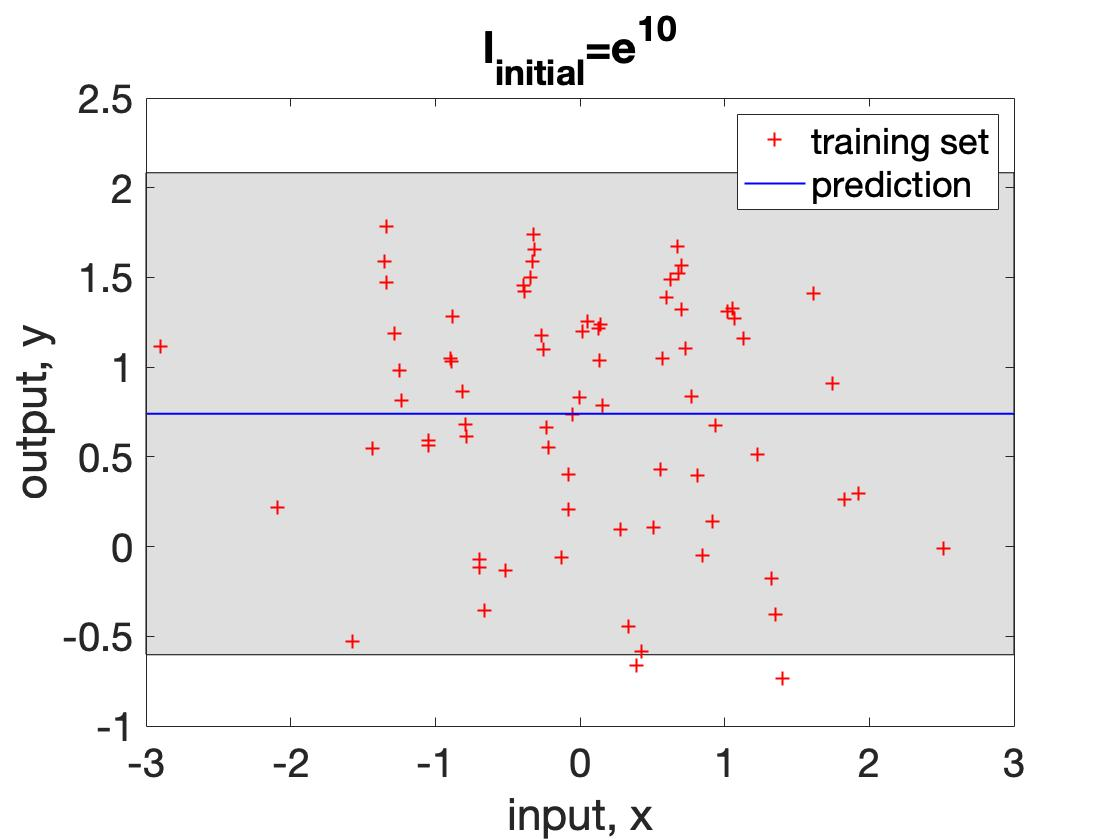
\includegraphics[width=.48\linewidth]{figures/b2.jpg}
	\caption{Functions obtained by modifying the initial hyperparameters (left to right: $log(l)=0$ and $log(l)=10$)}
	\label{fig:2}
\end{figure}
\noindent
In both cases, the predicted length scale is significantly higher (even higher than the test range) which results in a smooth function and a large noise standard deviation that is now comparable to the standard deviation of the model. In this case, the obtained model is too simple and can't really capture any "structure" in the data which is why we have noise everywhere. When the length scale increases further, the smoothness of the underlying function increases until the model becomes a "linear" function of slope $\sim\,0$ which corresponds to the average of the training data set.\\
To understand this behavior futher, both the lengthscale and the standard deviation of the noise are varied to cover a larger range of values (40 points each), while the standard deviation of the signal is kept constant ($\nu=1$) as illustrated in \hyperref[fig:2]{\textbf{Figure 3}}.
\[
log(l) \in [-4, 10] \,\,\,;\,\,\, log(\sigma_{noise}) \in [-5,2]
\]
\begin{figure}[H]
	\centering
	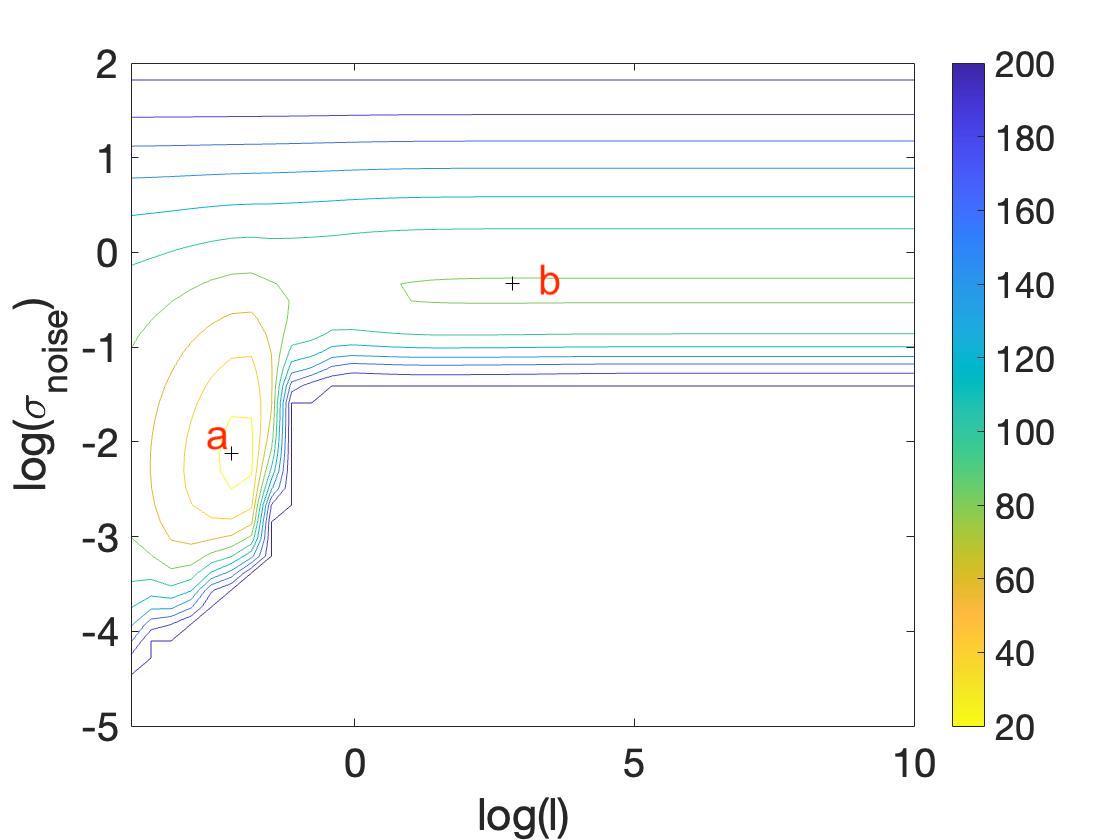
\includegraphics[width=.6\linewidth]{figures/b_contour_fixed.jpg}
	\caption{Negative log marginal likelihood (cf. colorbar) as a function of the lengthscale and noise standard deviation, both in log scale. Local minima are highlighted with '$+$' sign. (The values of $nlml \geq 200$ are set to 200 for an improved visibility.)}
	\label{fig:3}
\end{figure}
\noindent
We notice the presence of two local minima (denoted by the plus sign) in \hyperref[fig:3]{\textbf{Figure 3}}. The first (point a) corresponds to a region with low noise and small lengthscale, while the second (point b) corresponds to a region with higher noise and larger lengthscale. Indeed, a quick calculation yields the following values:

	\begin{table}[H]
	\centering
	\begin{tabular}{| c  | c | c | c |}
		\hline
		\textbf{Point} & \textbf{$l$} &  \textbf{$\sigma_{noise}$}& $likelihood$ \\
		\hline \hline
		\textbf{'a'} & 0.1102 & 0.1191  & 5.098e-7\\
		\hline
		\textbf{'b'} & 16.7855 & 0.7165 & 6.46e-35 \\
		\hline
	\end{tabular}
	\caption{Hyperparameters associated with each point. The standard deviation of the signal is fixed here ($\nu = 1$).}
	\end{table}
\begin{figure}[h]
	\centering
	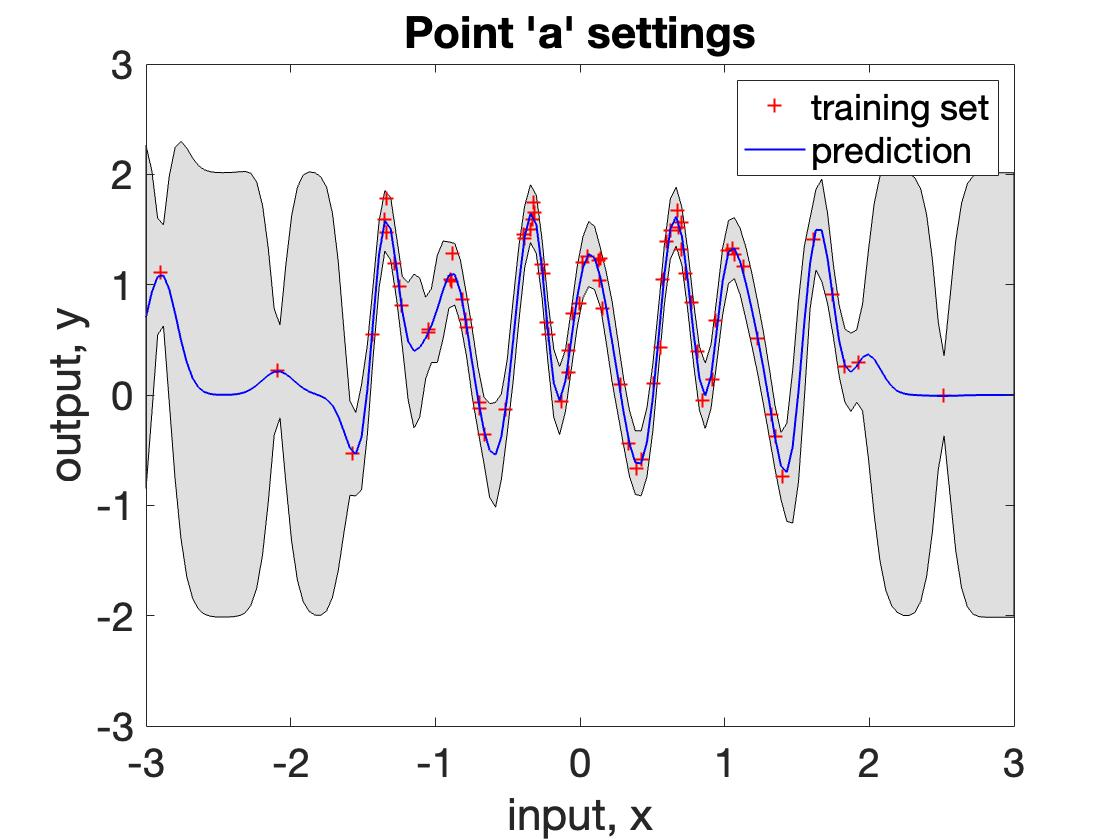
\includegraphics[width=.48\linewidth]{figures/bpointa.jpg}
	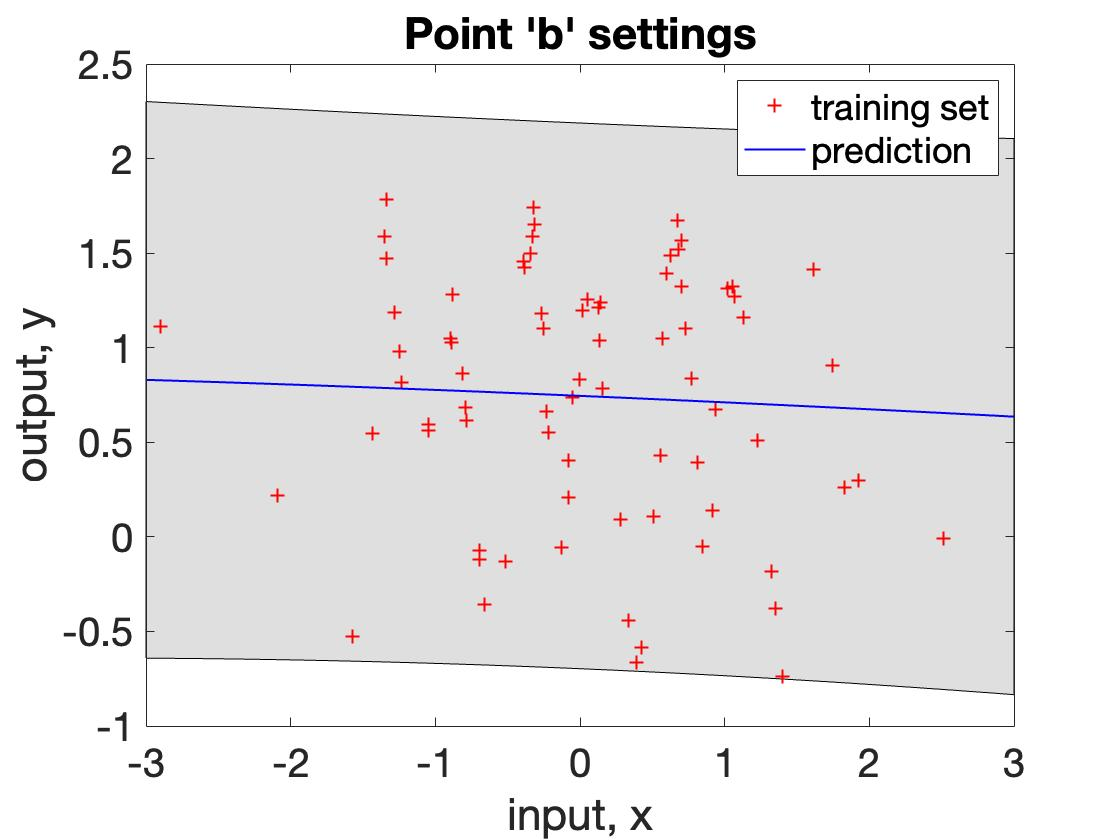
\includegraphics[width=.48\linewidth]{figures/bpointb.jpg}
	\caption{Functions obtained by using the hyperparameter settings for point 'a' and 'b' respectively}
	\label{fig:4}
\end{figure}
By plotting the models associated with the hyperparameters of each point, we obtain the functions in \hyperref[fig:4]{\textbf{Figure 4}}. This confirms our initial observation and highlights the presence of a second optimum which corresponds to the hyperparameters of point b. When the lengthscale is large, we notice that the marginal likelihood becomes almost independent of the lengthscale but that is compensated by a larger noise term: the model explains the data as noise everywhere(point b). Conversely, when the lengthscale decreases, the marginal likelihood becomes less and less dependent on noise (point a, also result of the previous question) because the model is able to explain the data.\\
For all these reasons, and knowing it maximises the likelihood ($lik(a)/lik(b) \sim 10^{28}$), it is reasonable to suggest that the fit associated with point 'a' in \hyperref[fig:4]{\textbf{Figure 4}} (or in the previous question, \hyperref[fig:1]{\textbf{Figure 1}}) is better.
\begin{lstlisting}
	% coursework1b.m
	for xx in range(linspace(-4,10,40))
		for yy in range(linspace(-5,2,40)):
			hyp = struct('mean', [] , 'cov', [xx(i),0] , 'lik', yy(j))
			nlml=gp(hyp, @infGaussLik, meanfunc, covfunc, likfunc, x, y);
			Z(j,i)=min(nlml,200)
		end
	end
	[X,Y] = meshgrid(xx,yy)
	contour(X,Y,Z);
\end{lstlisting}
\section*{Question (c)}
The data is \texttt{cw1a.mat} is now used to train a GP of periodic covariance function. We obtain the following results:
	\begin{table}[H]
	\centering
	\begin{tabular}{| c  | c | c | c | c | c |}
		\hline
		& \textbf{$l$} & $p$ &$\sigma$ &  \textbf{$\sigma_{noise}$} & $likelihood$  \\
		\hline \hline
		\textbf{Initial} & 1 & 1 & 1 & 1 &  2.8391e-35 \\
		\hline
		\textbf{covPeriodic predic.} & 1.0447 & 0.9988 & 0.9988 & 0.1094 &  2.0381e+15\\
		\hline \hline
		\textit{covSEiso predic.} &\textit{0.1282} & \textit{-}  & \textit{0.8970} & \textit{0.1178} & 6.7971e-06\\
		\hline
	\end{tabular}
	\caption{Initial and predicted hyperparameters}
\end{table}
\begin{figure}[h]
	\centering
	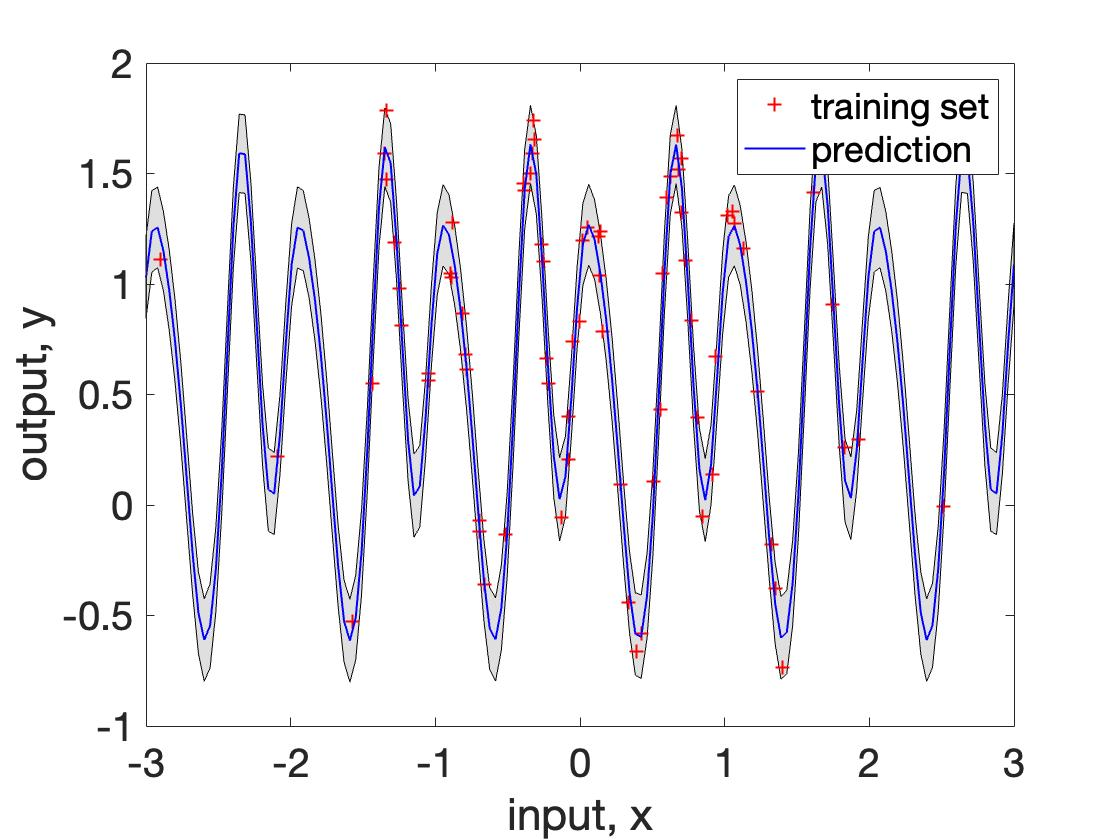
\includegraphics[width=.6\linewidth]{figures/c1.jpg}
	\caption{Training and predicted fit using a periodic covariance function (\textit{note: })}
\end{figure}
The obtained error bars are in this case relatively small compared to the ones obtained using a square-exponential covariance, even in low populated regions. This makes sense since using a periodic covariance function implies that:
\[
k(x_1,x_2)=k(x_1,x_3)\,\,\, if \,\,\, | x_1 - x_2 | \equiv | x_1 -x_3| \, \,[p]
\]
where p is the period and supposing $x_1 \neq x_2 \neq x_3$.\\
The error bars are also almost constant everywhere because we have in this case $p\sim l$ which results in a model that is neither too simple (smooth function, higher noise) nor too complex (very wiggly, overfitting).
The standard deviation of the noise is relatively smaller which suggests that the error bars are most likely due to the uncertainty of the model which is also smaller than the $covSEiso$ one. Overall, the fit gives off a good impression and its likelihood is considerably higher than the one obtained using $covSEiso$ which suggests that the data-generating mechanism is likely periodic.
\begin{lstlisting}
	% coursework1c.m
	covfunc = @covPeriodic;
	hyp_min = minimize(hyp, @gp, -100, @infGaussLik, meanfunc, covfunc, likfunc, x, y);
	[ys stds] = gp(hyp_min, @infGaussLik, meanfunc, covfunc, likfunc, x, y, xs);
\end{lstlisting}
\section*{Question (d)}
We generate a random data set in the given range of x-values, then we train a GP with a periodic-SEiso product composite kernel. The result is illustrated in \hyperref[fig:6]{\textbf{Figure 6}}.
\begin{figure}[H]
	\centering
	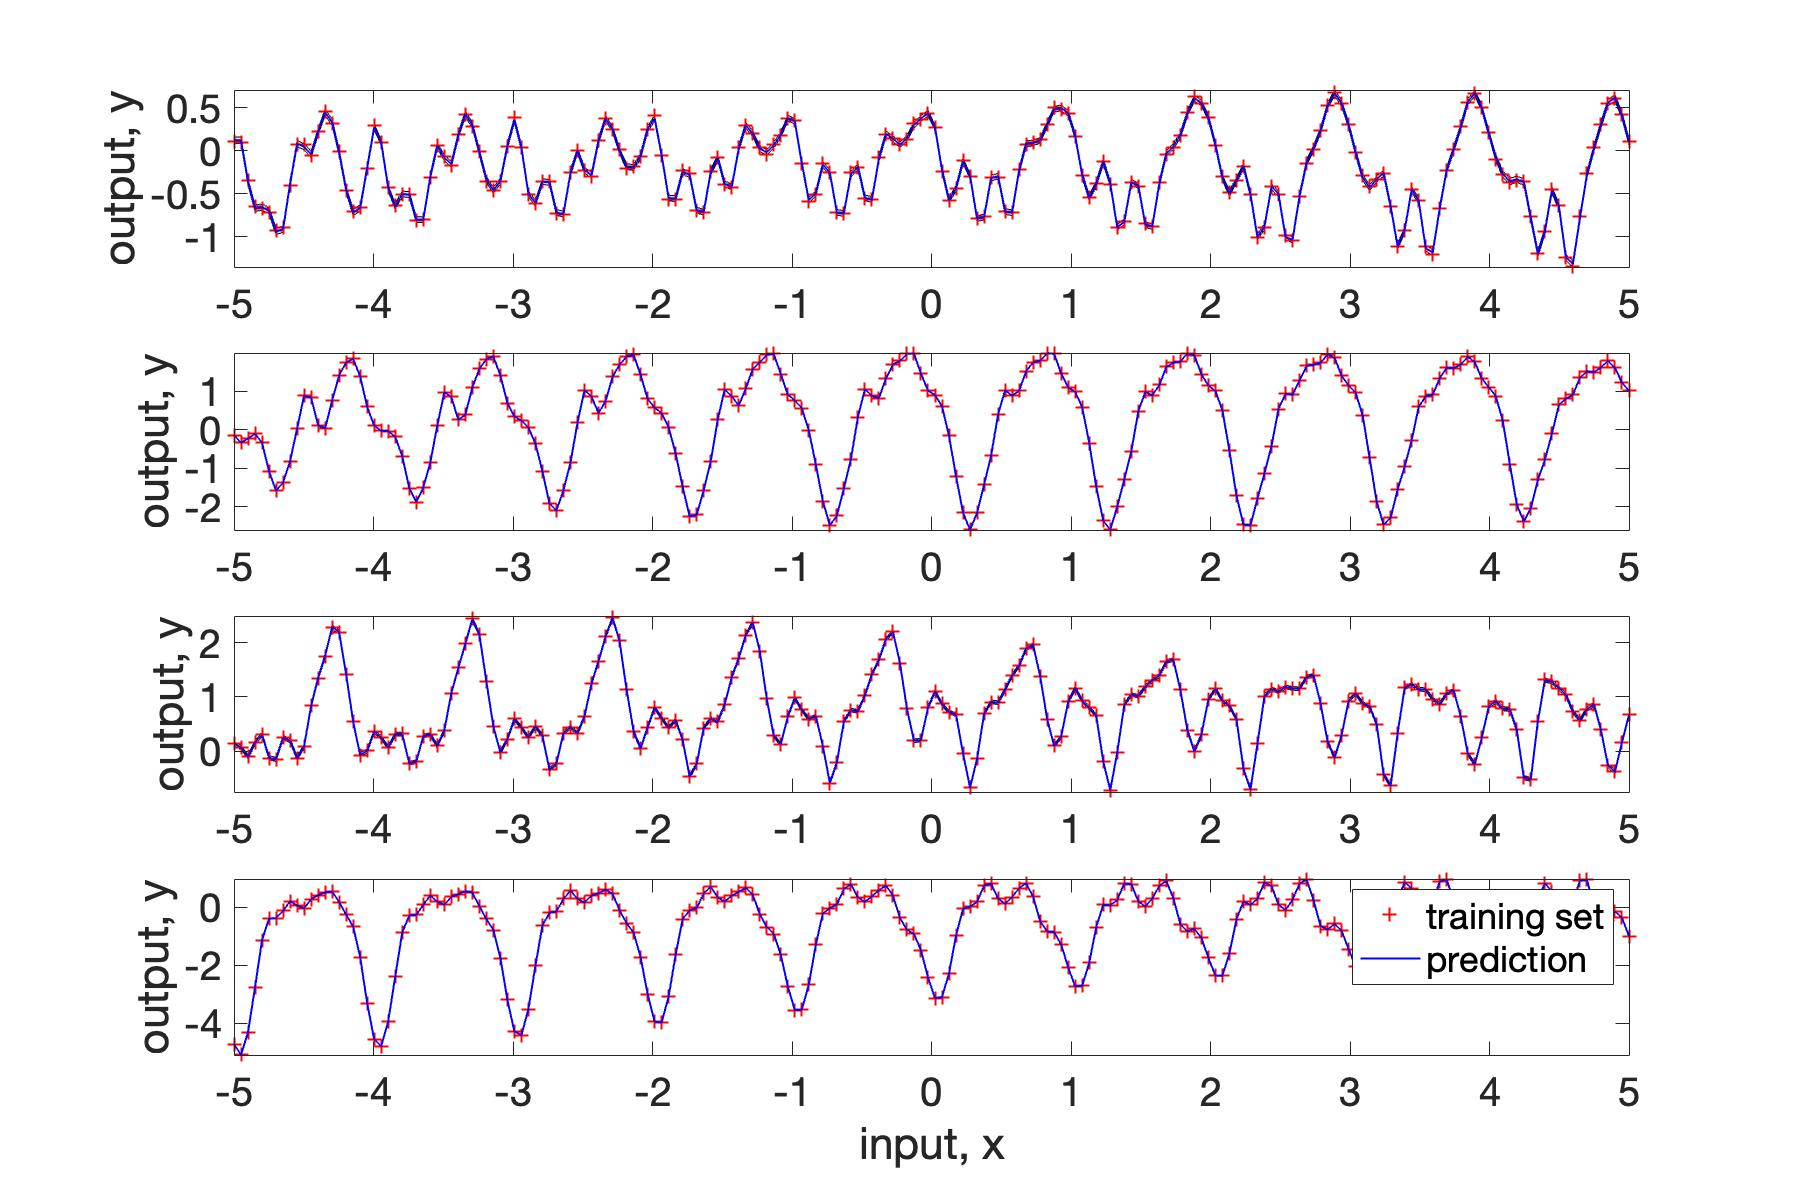
\includegraphics[width=\linewidth]{figures/d1.jpg}
	\caption{Functions obtained for different seeds (0.01, 0.1, 0.5, and 1 top-down) using random x data.}
	\label{fig:6}
\end{figure} 
In order to apply Cholesky's decomposition to the covariance matrix, it should positive definite, hence the need to add the given diagonal matrix.\\
We observe that the functions in each case look like a combination of SEiso covariance (hump-like structure) and periodic covariance (repetitions over a period of 1). The composite kernel, therefore, combines the properties of both covariances. We notice we obtain a wide variety of functions when changing the seed but they all keep the properties of the two kernels. The period is approximately one which is consistent with the value calculated too. Because the lengthscale ($l \approx 0.7$) is 70\% smaller than the period ($p\approx1$), there is a small offset which "breaks" the periodic aspect of the function in certain humps.
\begin{lstlisting}
	% coursework1d.m
	se=[.01 .1 .5 1]
	for i=1:length(se)
		covfunc = {@covProd, {@covPeriodic, @covSEiso}};
		hyp.cov = [-0.5 0 0 2 0];
		x = linspace(-5,5,200)';
		K = feval(covfunc{:},hyp.cov, x);
		K_pos_def=K+1e-6*eye(200)
		y = chol(K_pos_def)'*gpml_randn(se(i), 200, 1);
		plot subplot
	end
\end{lstlisting}
\section*{Question (d)}

	
	
	
	
	
\end{document}
